% ---------------------- setting ---------------------- %
\documentclass[10pt,landscape,a4paper]{article}
\input{../Math.tex}
\usepackage[margin=0.2in]{geometry}
\usepackage{multicol}
\usepackage{fancyhdr}
\usepackage{amsmath, amsfonts, mathtools, amsthm, amssymb, mathrsfs}
\usepackage{lipsum}

\setlength\parindent{0pt}

\setlength{\columnseprule}{0.5pt}
\pagestyle{fancy}
\renewcommand{\headrulewidth}{0pt}
\fancyhf{}
\pagestyle{empty}

\makeatletter
\renewcommand{\section}{\@startsection{section}{1}{0mm}%
                                {-1ex plus -.5ex minus -.2ex}%
                                {0.5ex plus .2ex}%x
                                {\normalfont\large\bfseries}}
\renewcommand{\subsection}{\@startsection{subsection}{2}{0mm}%
                                {-1explus -.5ex minus -.2ex}%
                                {0.5ex plus .2ex}%
                                {\normalfont\normalsize\bfseries}}
\renewcommand{\subsubsection}{\@startsection{subsubsection}{3}{0mm}%
                                {-1ex plus -.5ex minus -.2ex}%
                                {1ex plus .2ex}%
                                {\normalfont\small\bfseries}}
\makeatother

\makeatletter
\g@addto@macro\normalsize{%
  \setlength{\abovedisplayskip}{2pt}%
  \setlength{\belowdisplayskip}{2pt}%
  \setlength{\abovedisplayshortskip}{2pt}%
  \setlength{\belowdisplayshortskip}{2pt}%
}
\makeatother

\begin{document}
\begin{multicols}{3}
% ---------------------- Content ---------------------- %
Peter Chen's \textbf{Entity-Relationship (ER) Model}

\textbf{\underline{Cardinality constraint (\(\to\) from \(\square\) to \(\diamondsuit\))}}:

\textbf{Total Participation}: all entity in set must participate in at least one relationship, \textcolor{red}{double line}; \textbf{Partial}: an entity in the entity set may not participate in any relationship.

\textbf{Multi-value attributes}: more than one value, \textcolor{red}{double ellipse}; \textbf{Composite attributes}: can be divided into smaller subparts; \textbf{Derived attributes}: values can be derived from other attributes (\textcolor{red}{dashed ellipse})

\textbf{\underline{Keys}}: \textcolor{red}{underlined attributes}; \textbf{Super-key}: any set of attributes that can uniquely identify entity; \textbf{Candidate key}:  minimal set of attributes whose values uniquely identify an entity in the entity set; \textbf{Primary key}: candidate key chosen to serve as the main key; \textbf{Surrogate key}: system-generated value; \textbf{Partial (discriminator) key}: uniquely identifies weak entities within the context of the identifying entity (\textcolor{red}{dashed underline})

\textbf{Weak entity sets}: no primary key, dependent, represented by a \textcolor{red}{double rectangle}, must be related to the identifying entity set via a total one-to-many relationship; \textbf{identifying relationship} is represented by a \textcolor{red}{double diamond}.

\textbf{\underline{Relationship key}}

\textbf{1:1}: both keys can serve as keys for relationship

\textbf{1:N}: use key from `many' side

\textbf{M:N}: primary key is the union of the primary keys 

\textbf{\underline{Class Hierarchies}}

\textbf{Overlap constraints}: whether multiple subclasses are allowed to contain the same entity. \textbf{Covering constraints}: whether the entities in the subclasses collectively include all entities in the super-class.  

\textbf{\underline{Crows Feet Notation}}

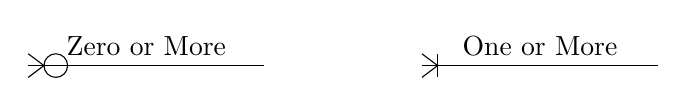
\begin{tikzpicture}
  \draw (0,0) -- (3,0);
  \draw (0,0.15) -- (0.2,0) -- (0,-0.15);
  \draw (0.35,0) circle (0.15);
  \node[above] at (1.5,0) {Zero or More};
  \draw (5,0) -- (8,0);
  \draw (5,0.15) -- (5.2,0) -- (5,-0.15);
  \draw (5.2,0.15) -- (5.2,-0.15);
  \node[above] at (6.5,0) {One or More};
\end{tikzpicture}

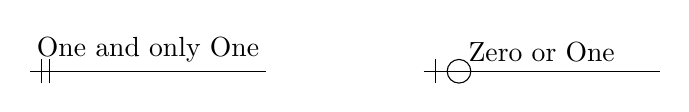
\begin{tikzpicture}
  \draw (0,0) -- (3,0);
  \draw (0.15,0.15) -- (0.15,-0.15);
  \draw (0.25,0.15) -- (0.25,-0.15);
  \node[above] at (1.5,0) {One and only One};

  \draw (5,0) -- (8,0);
  \draw (5.15,0.15) -- (5.15,-0.15);
  \draw (5.45,0) circle (0.15);
  \node[above] at (6.5,0) {Zero or One};
\end{tikzpicture}

\textbf{\underline{Relation Model and mapping}}

\textbf{Step 1}: For strong entity \(E\), create new relation \(R\). \(R\) include all simple attributes (and simple components of composite attributes) of \(E\). PK of \(R\) is key of \(E\).  

\textbf{Step 2}: For weak entity \(W\) with the identifying entity type \(E\), create new relation \(R\). \(R\) include all simple attributes (and simple components of composite attributes) of \(W\), primary key attributes of the relation derived from \(E\). PK is the combination of the foreign key to \(E\) and the partial key of \(W\).

\textbf{Step 3 1-to-1}: For relationship \(B\), let \(S\) and \(T\) be the participating entity. Choose one of them (say \(S\)) — preferably the one with total participation. Add PK attributes of \(T\) to relation \(S\) as a foreign key. Add all simple attributes (and simple components of composite attributes) of \(B\) to \(S\). 

\textbf{Step 4 1-to-M}: For relationship \(B\), let \(S\) and \(T\) be the participating entity, where \(S\) is on the ``one'' side and \(T\) on the ``many'' side. Add to relation \(T\) the PK attributes of \(S\) as a FK. Add any simple attributes (or simple components of composite attributes) from the relationship \(B\). 

\textbf{Step 5 M-to-N}: For relationship \(B\), let \(S\) and \(T\) be the participating entity. Create new relation \(R\). Attributes of \(R\) include the PK attributes of \(S\) and \(T\), and all simple attributes (and simple components of composite attributes) of \(B\). The PK of \(R\) is the combination of the keys of \(S\) and \(T\).

\textbf{Step 6}: For multivalued attribute \(A\) of entity \(E\), create new relation \(R\). If \(A\) is simple attribute, attributes of \(R\) are \(A\) and the PK of \(E\) (as FK). If \(A\) is composite attribute, the attributes of \(R\) are all simple components of \(A\) and the PK of \(E\) (as FK). PK of \(R\) is the combination of all attributes in \(R\).  

\textbf{Step 7}: For \(n\)-ary relationship type (\(n > 2\)), create new relation \(R\) using the same approach as for M-to-N relationships. If one of the participating entity types has a participation ratio of 1, its key may serve as the primary key for \(R\).  

\textbf{\underline{Relational Integrity Constraints}}

\textbf{Key constraint:} Candidate key values must be unique

\textbf{Entity integrity:} PK cannot be \texttt{NULL} 

\textbf{Referential integrity:} FK is \texttt{NULL} or exist

\textbf{\underline{Relational Algebra (\(\land\) AND, \(\lor\) OR, \(\lnot\) NOT)}}

\textbf{Select}: \(\sigma_P(r) = \{\ t \mid t \in r \land P(t) \ \}\); \textbf{Project}: \(\Pi_{A_1, A_2, \dots, A_k}(r)\)

\textbf{Union}: \(r \cup s = \{\ t \mid t \in r \lor t \in s \ \}\), duplicate tuples are eliminated in the result. Union-compatible: have the same no. of attributes and same domains.

\textbf{Set difference}: \(r - s = \{\ t \mid t \in r \land t \notin s \ \}\)

\textbf{Cartesian-Product}: \(r \times s = \{\ pq \mid p \in r \land q \in s\ \}\) (R concatenate S, \(\vert R \vert \times \vert S \vert\) rows). 

\textbf{Rename}: \(\rho_X(E)\); Tmp Assignment: \texttt{<name> \(\leftarrow\) <E>}. Assignment simply allows us to store intermediate results under a temporary name for convenience — it does not modify the relations themselves or affect the algebraic computation.

\textbf{Set-intersection}: \(r \cap s = \{\ t \mid t \in r \land t \in s\ \} = r - (r - s)\)

\textbf{Natural join}: \(r \Join s\), if have attributes in common, find same value rows. If nothing in common, simply cartesian product

\textbf{Division}: returns the set of all \(x\) values such that for every \(y\) value in a tuple of \(B\), there exists a tuple \(\langle x, y \rangle\) in \(A\).
\[
A / B = \Pi_x(A) - \Pi_x\big( (\Pi_x(A) \times B) - A \big)
\]

\textbf{Theta join}: \(r \Join_{\theta} s = \sigma_{\theta}(r \times s)\), \(\theta\) is join condition. Equijoin is theta join with only \((=)\). 

\textbf{\underline{Equivalence Rules}}

1. Conjunctive selection can be deconstructed into a sequence of individual selections: \(\sigma_{\theta_1 \wedge \theta_2} (E) = \sigma_{\theta_1} (\sigma_{\theta_2} (E))\)

2. Selection is commutative: \(\sigma_{\theta_1} (\sigma_{\theta_2} (E)) = \sigma_{\theta_2} (\sigma_{\theta_1} (E))\)

3. Only last in a sequence of projections is needed: \(\Pi_{L_1}(\Pi_{L_2}(\dots(\Pi_{L_n} (E)))) = \Pi_{L_1} (E)\)

4. Selections can combined with Cartesian and theta joins: \(\sigma_{\theta} (E_1 \times E_2) = E_1 \Join_{\theta} E_2\), \(\sigma_{\theta_1} (E_1 \Join_{\theta_2} E_2) = E_1 \Join_{\theta_1 \wedge \theta_2} E_2\) 

5. Theta-join are commutative: \(E_1 \Join_{\theta} E_2 = E_2 \Join_{\theta} E_1\) 

6. Natural join are associative: \((E_1 \Join E_2) \Join E_3 = E_1 \Join (E_2 \Join E_3)\);  Theta joins are associative, where \(\theta_2\) involves attributes from only \(E_2\) and \(E_3\): \((E_1 \Join_{\theta_1} E_2) \Join_{\theta_2 \wedge \theta_3} E_3 = E_1 \Join_{\theta_1 \wedge \theta_3} (E_2 \Join_{\theta_2} E_3)\)

7. Selection distributable over theta join under 2 conditions:

a. \(\theta_0\) involve only one of the expressions (\(E_1\)) being joined: \(\sigma_{\theta_0} (E_1 \Join_{\theta} E_2) = (\sigma_{\theta_0} (E_1)) \Join_{\theta} E_2\) 

b. when \(\theta_1\) involve only \(E_1\), \(\theta_2\) involve only \(E_2\): \(\sigma_{\theta_1 \wedge \theta_2} (E_1 \Join_{\theta} E_2) = (\sigma_{\theta_1} (E_1)) \Join_{\theta} (\sigma_{\theta_2} (E_2))\) 

8. Projection distributes over the theta join: a. \(\theta\) involve only \(L_1 \cup L_2\): \(\Pi_{L_1 \cup L_2} (E_1 \Join_{\theta} E_2) = (\Pi_{L_1} (E_1)) \Join_{\theta} (\Pi_{L_2} (E_2))\) 

b. \(L_3\) from \(E_1\), involve in \(\theta\), not in \(L_1 \cup L_2\), and \(L_4\) from \(E_2\), involve in \(\theta\), not in \(L_1 \cup L_2\). Then \(\Pi_{L_1 \cup L_2} (E_1 \Join_{\theta} E_2) = \Pi_{L_1 \cup L_2} ((\Pi_{L_1 \cup L_3} (E_1)) \Join_{\theta} (\Pi_{L_2 \cup L_4} (E_2)))\) 

\textbf{\underline{Heuristic Optimization}}: Reduce no. of choices that must be made in a cost-based fashion. Perform selection and projection as early as possible. Cost-based query optimization: Generate equivalent expressions using rules; get alternative query plans; choose cheapest plan using estimation

no. of join orders \(= (2(n - 1))!/(n - 1)!, \text{ for } r_1, \dots, r_n\) 

Left-deep join preferred because more efficient

\textbf{\underline{Join Algorithm}}

Nested loop join can be used with any kind of join conditions but expensive. Coarse-grain parallel machine has few powerful processors; Massively parallel or fine grain parallel machine use thousands of processors. 

Throughput: no. of tasks completed in a given time interval; Response time: amount of time to complete a task

Intraoperation: parallelize each individual operation in query; Interoperation: execute different operations in parallel, can increase throughput

Hash Join Algo: Partition relations using hash function, joins two tables by hashing the join key of the smaller table into memory and then probing it with tuples from the larger table. Output concatenation. Relations must be partitioned on join attributes, using same hash function. 

\textbf{\underline{SQL}}: Data Manipulation Language (DML); Data Definition Language (DDL); Triggers and Advanced Integrity Constraints. SQL allows duplicates in relations and query results

\texttt{HAVING} is used to qualify a \texttt{GROUP BY} clause. \texttt{WHERE} filters rows before grouping, \texttt{HAVING} filters groups after aggregation.

\textbf{\underline{Functional Dependency}}

lossless-join decomposition (non-additive join): 

\(r = \Pi_{R_1} (r) \bowtie \dots \bowtie \Pi_{R_n} (r)\)

lossless-join decomposition if only decompose into \(R_1, R_2\):
\[
  (R_1 \cap R_2) \to R_1 \in F^+ \quad OR \quad (R_1 \cap R_2) \to R_2 \in F^+
\]
Dpdncy Preservation: \(((\Pi_{R_1} (F)) \cup \cdots \cup (\Pi_{R_m} (F_m)))^+ = F^+\)

def \(\alpha \to \beta\) : when \(t_1, t_2\) agree on \(\alpha\), they agree on \(\beta\) 

Set of all FDs implied by a given set \(F\) of FDs is called the closure
of \(F\), denoted as \(F^+\); Attribute closure \(A^+\) is the set of attributes that are functionally determined by \(A\) under \(F\). 

\textcolor{blue}{Armstrong's Axioms:} sound: generate only FDs that hold in \(F^+\); complete: generate all FDs in \(F^+\) 

1. Reflexivity: if \(Y \subseteq X\), then \(X \to Y\); \textcolor{red}{trivial}

2. Augmentation: if \(X \to Y \models XZ \to YZ\) 

3. Transitivity:  if \(\{X \to Y, Y \to Z\} \models X \to Z\) 

4. Additivity: if \(\{X \to Y, X \to Z\} \models X \to YZ\) 

5. Projectivity: if \(\{X \to YZ\} \models \{X \to Y, X \to Z\}\)

6. Pseudo-transitivity: if \(\{X \to Y, ZY \to W\} \models XZ \to W\) 

\(\alpha\) is super key iff. \(\alpha \to R\); \(\alpha\) is candidate key iff. \(\alpha \to R\) and \(\forall \gamma \subseteq \alpha\ s.t.\ \gamma \nrightarrow R\) (minimal property)

\textbf{Algo TEST Lossless Join}: Create matrix \(S\), initially cols are attributes, rows are subsets. Put \(a\) in cells where the corresponding subsets contain corresponding attributes, other put \(b\). Repeat the following process till \(S\) has no change or one row is made up entirely of \(a\) symbols (then lossless).

For each \(X \to Y\), choose the rows where the elements corresponding to \(X\) take the value \(a\). In those chosen rows (must at least two rows), the elements corresponding to \(Y\) also take the value \(a\) if one of the chosen rows take the value \(a\) on \(Y\).

\textbf{\underline{Minimal Cover}}

\(F\) cover \(E\) if \(E \subseteq F^+\). Equivalent if \(E^+ = F^+\). Min cover \(F_{\min}\) of \(E\) is the min set of dp that is equivalent to \(E\). FD is min if \(X \to Y\), \(Y\) consists of a single attr.; left-reduced s.t. no \(A \in X, A \to Y\); cannot reduce. \textbf{Algo Min Cover}: Reduce right, left (find attribute closure) then redundant FDs. 

\textbf{3NF Decomposition Algorithm}: Find a minimal cover \(G\) of \(F\); for each left-hand side \(X\) in \(G\), create a relation schema containing \(X\) and all attributes functionally determined by \(X\); if no relation contains a key of \(R\), add one relation with a key of \(R\); finally, remove redundant (subsumed) relations.

\textbf{\underline{Normal Form}}

\textbf{Prime attribute}: member of candidate key; \textbf{Full functional dependency} of Y: \(X \to Y \text{ and } \forall Z \subset X \text{ s.t. } Z \nrightarrow Y\). \textbf{Transitive dependency}: \(X \to Y\) is transitive if \(Z\) is not prime, \(X \to Z \to Y\) 

1NF: Repeating groups are not permitted

2NF: Each non-key attribute in the table must be dependent on the entire primary key. (no partial key dependency)

3NF: Each non-key attribute in the table must depend on the key, the whole key, and nothing but the key. (no transitive), i.e. no `not superkey' \(\to\) `nonprime'

BCNF: Each attribute in the table must depend on the key, the whole key, and nothing but the key, i.e. only have `superkey' \(\to\) `prime' or `nonprime'

4NF: The only kinds of multivalued dependency allowed in a table are multivalued dependencies on the key.

5NF: It must not be possible to describe the table as being the logical result of joining some other tables together.
\[
  1NF \supset 2NF \supset 3NF \supset BCNF \supset 4NF \supset 5NF
\]

\textbf{\underline{Transaction}}

Atomicity: all or nothing, no partial update; Consistency: remain in valid state; Isolation: transaction doesn't affect each other; Durability: permanent change after commit; 

Conflict: both access same item, at least one write. Conflict equivalent if two schedules involve same actions of same transactions and every pair of conflicting actions is ordered same way. If a schedule can be transformed by a series of swaps of non-conflicting instructions, they are conflict equivalent, then conflict serializable. Any conflict serializable schedule is also a serializable schedule. 

Determine conflict serializability: Draw precedence graph; Check if the graph is cyclic, cyclic then non-serializable. Draw edge \(T_i \to T_j\) if conflict and \(T_i\) access data earlier. If acyclic, serializability order can be obtained by topological sorting. 

Exclusive Lock / X Lock / Write Lock: read or write data; Shared Lock / S Lock / Read Lock: read only. Lock is compatible only when both are S lock. 

Simple lock: unlock after last ops. 2 phase lock: Growing phase: lock and not release; Shrinking phase: release locks and not obtain new locks (guarantee serializability)

Deadlock with timeout: longer than timeout then abort; Timestamp TS: assume \(T_i\) request lock, \(T_j\) hold lock. \textbf{Wait-Die}: if \(T_i\) older, wait; if \(T_i\) younger, abort. \textbf{Wound-wait}: if \(T_i\) younger, wait; if \(T_i\) older, abort. 

\textbf{\underline{Buffer}}

DBMS stored on disk. Process data: CPU and I/O cost.

Access time: read/write request issued; Seek time: time to reposition arm over correct track; Rotational latency: time for sector to appear under head; Data-transfer rate. 

Buffer pool: portion of main mem available to store copies of disk blocks. No I/O cost between app and MM

If data in buffer, return addr in MM, no IO; Not in buffer, read disk. 

\textbf{\underline{Recovery}}

Input: data from disk to main memory; Output: reverse

Log-Based Recovery: \(\langle T_i \text{ start} \rangle\), before execute \texttt{write(X)}, \(\langle T_i, X, V_1, V_2 \rangle\), \(V_1\) is value before write, \(V_2\) is new value; \(\langle T_i \text{ commit} \rangle\) when finish last statement.

Immediate DB modification: allow update to butter / disk before commit; log must be written before db item is written

Log record buffering: log buffered in MM. Output to stable storage when block is full / log force op. Log force: commit a transaction by forcing all logs into stable storage. Log buffered in order of creation, transaction only commit after log \(\langle commit \rangle\). Write-ahead logging: all log output to stable storage, then output data to db. UNDO (log hv start only): set value of item to old value; must in reverse order from log. REDO (log hv start and commit): redo write, set value to new value. 

Redo Algo: find last checkpoint start redo forward, for \(\langle T_i, X_j, V_1, V_2 \rangle\) do \(\langle T_i, X_j, V_2 \rangle\) (no need write for abort or commit); Undo: Rollback from end, for each log \(\langle T_i, X_j, V_1, V_2 \rangle\), undo by \(\langle T_i, X_j, V_1 \rangle\), finally \texttt{abort}

Checkpoint: log and data both output. 

Deferred DB modification: write after commit; redo only committed.

\hrulefill

A set of transaction must have conflict serializable schedule (serial)

Result equivalence provide same result, not conflict equivalence

% ---------------------- END ---------------------- %
\vfill\break
\end{multicols}
\end{document}